\begin{table}[htb]
  \centering
  \caption{Resource usage by entity, including resources used by sub-entities.}
  \begin{tabular}{llll}
    \toprule
                         & LC Combinationals & LC Registers & Memory Bits \\
    \midrule
    Fetch Stage          &  40          & 16       & 0            \\
    Decode Stage         &  165         & 1088     & 0            \\
    -- Register File     &  47          & 1040     & 0            \\
    Execute Stage        &  2143        & 153      & 0            \\
    -- ALU               &  412         & 0        & 0            \\
    Memory Stage         &  463         & 114      & 0            \\
    -- Memory Unit       &  53          & 0        & 0            \\
    Write-Back Stage     &  79          & 38       & 0            \\
    Forwarding Unit      &  14          & 0        & 0            \\
    Control Unit         &  3           & 0        & 0            \\
    \cmidrule{1-4}
    Sum (top)            &  3342        & 1703     & 262208       \\
    \bottomrule
  \end{tabular}
\end{table}

\begin{qa}
  \question{What is the maximum frequency of your design?}
  \answer{77,33 MHz}
  \question{Where is the critical path of your design?}
  \answer{The critical path exists between the Execute- and the Memory-Stage. (From rs1 through the forwarding units and the alu and as aluresult to the memory stage)}
  \begin{figure}[ht!]
  	\centering
  	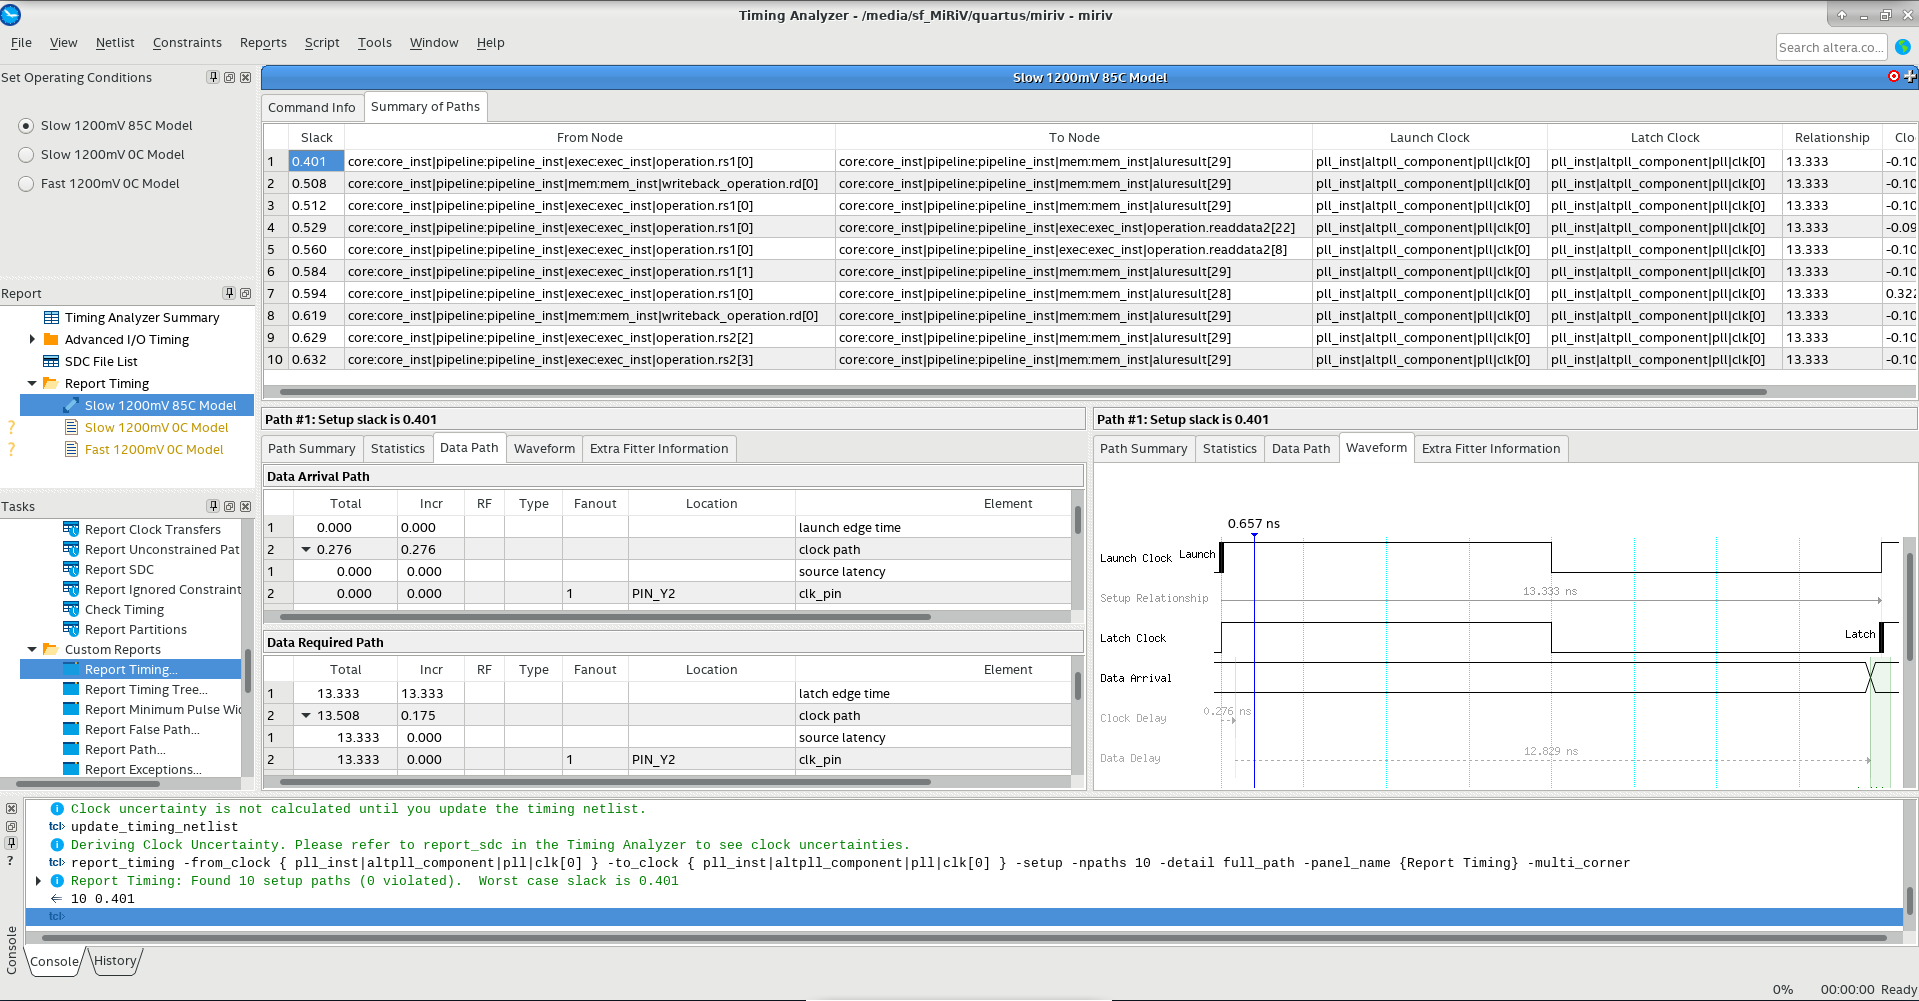
\includegraphics[width=1.0\linewidth]{img/criticalpath.png}
  	\caption{Quartus Timing Analyzer for critical path.}
  	\label{fig:sim2}
  \end{figure}
\end{qa}

